\pdfinfo{
/ModDate (\pdfcreationdate)                                   
/Producer (pdfLaTeX)                                    
}


\documentclass[fleqn,oneside,openany,a4paper,11pt]{book}

\usepackage{color}
\usepackage[utf8]{inputenc}
\usepackage[breaklinks]{hyperref} %
\usepackage{pracadok}
\usepackage{longtable}
\usepackage{float}

\pdfcompresslevel=9

\def\uwaga#1{}

\begin{document}
\let\s\lstinline
\lstset{inputencoding=utf8, extendedchars=true,literate={ą}{{\k{a}}}1 {ć}{{\'c}}1 {ę}{{\k{e}}}1 {ł}{{\l{}}}1 {ń}{{\'n}}1 {ó}{{\'o}}1 {ś}{{\'s}}1 {ż}{{\.z}}1 {ź}{{\'z}}1 {Ą}{{\k{A}}}1 {Ć}{{\'C}}1 {Ę}{{\k{E}}}1 {Ł}{{\L{}}}1 {Ń}{{\'N}}1 {Ó}{{\'O}}1 {Ś}{{\'S}}1 {Ż}{{\.Z}}1 {Ź}{{\'Z}}1}

% Tytuł
\def\autor{Informatyka Stosowana III rok}
\def\tytul{\textbf{\LARGE Zespołowe Przedsięwzięcie Inżynierskie}}
\def\promotor{~}
\def\miejscerokwydania{Nowy Sącz \today}
\def\nazwauczelni{PAŃSTWOWA WYŻSZA SZKOŁA ZAWODOWA}
\def\imienia{INSTYTUT  TECHNICZNY}
\def\wydzial{Kierunek Informatyka Stosowana}

\thispagestyle{empty}
{
\hbox{}\vskip 0.3\textheight
\hspace{1cm}
\centering
\vbox{
\noindent\textbf{\Huge Przygotowanie zdjęć do legitymacji studenckiej. \\ 
\
\noindent\textbf{\vspace{0.3cm}Zespołowe przedsięwzięcie inżynierskie}\\
\noindent\textbf{Prowadzący: Antoni Ligęza}}\\}
%\noindent e-mail: \verb|aligeza@pwsz-ns.edu.pl|\\
%\noindent \verb|http://www.pwsz-ns.edu.pl/aligeza|}\\}
\definecolor{tlo}{rgb}{.7,.7,.7} 
\lstset{language=bash,commentstyle=\scriptsize,backgroundcolor=\color{tlo},%
basicstyle=\scriptsize}

%spis tresci
{\footnotesize\tableofcontents}

\setcounter{chapter}{0}
%Opis wykonywanego zadania
%Cel
%Zakres prac
%Interesariusze

\chapter{Zespołowe przedsięwzięcie}

\begin{itemize}
\item Przygotowanie zdjęć do legitymacji studenckiej. 
\item Projekt jest odpowiedzią na uzasadnioną potrzebę istnienia narzędzia służącego do automatycznej edycji zdjęć, która ułatwi wydruk zdjęć do legitymacji
\end{itemize}

\section{Członkowie zespołu z określeniem funkcji}
\begin{description}
\item[1] Paweł Golonka - kierownik zespołu
\item[2] Karol Liszka - programista C\#	
\item[3] Bartosz Rusinek - tester aplikacji, autor pomocy, itp
\end{description}

\section{Uzasadnienie potrzeby realizacji projektu}
Projekt ma za zadanie pomóc nowym studentom w przygotowaniu zdjęć do legitymacji czy też do innego użytku. Utworzenie stosownej aplikacji pozwoli na ominięcie kosztów związanych z wykonaniem zdjęcia u profesjonalnego fotografa a także umożliwi łatwe przygotowanie zdjęcia do wysłania w formie elektronicznej. Narzędzie to pozwoli również na tworzenie gotowych  bloków zdjęć w wybranej przez użytkownika wielkości.


\section{Cele projektu}

Zespołowe przedsięwzięcie inżynierskie obejmuje przygotowanie aplikacji dla Państwowej Wyższej Szkoły Zawodowej wspomagającej proces przygotowanie fotografii przeznaczonych do legitymacji studenckiej. Program ma pobierać zdjęcie w jednym z wymienionych formatów, a następnie wykadrować wybrany element oraz zapisać go do podanych rozmiarów. 
W dalszym etapie, jego zadaniem będzie utworzenie bloku zdjęć w oparciu o parametry podane przez użytkownika.

\section{Grupy docelowe}
Odbiorcą aplikacji jest PWSZ w Nowym Sączu - Instytut Techniczny a sama aplikacja dedykowana jest dla studentów. 

\section{Zakres projektu}
\textbf{Etapy, które zostaną zrealizowane aby uzyskać postawiony cel}
\begin{enumerate}
\item Wywiad ze zleceniodawcą - zapoznanie się z oczekiwaniami co do aplikacji.
\item Przygotowanie środowiska do pracy z dokumentami \LaTeX oraz C\#.
\item Opracowanie programu w języku C\#
\item Opracowanie plików pomocy i szaty graficznej programu.
\item Kompilacja raportów do formatu PDF, utworzonych w \LaTeX. 
\end{enumerate}


\section{Struktura podziału prac (zadań) - WBS}
\textbf{Hierarchiczna dekompozycja projektu na zadania i aktywności.}
\begin{enumerate}
\item{Wybranie tematu projektu.}
\item Zebranie informacji w wywiadzie ze zleceniodawcą.
\begin{enumerate}
\item Informacje o celach programu.
\item Informacje na temat sposobu działania.
\item Informacje na temat wyniku który ma zostać zwrócony. 
\end{enumerate}
\item{Organizacja pracy}
\begin{enumerate}
\item Wybranie lidera grupy.
\item Wstępny podział obowiązków pośród członków grupy.
\item Określenie języka programowania oraz środowiska w którym program zostanie zaimplementowany.
\end{enumerate}
\item Przygotowanie środowiska
\begin{enumerate}
\item Instalacja i konfiguracja środowiska LaTeX oraz edytora Texmaker.
\item Utworzenie i konfiguracja repozytorium.
\item Instalacja Microsoft Visual Studio 2013.
\end{enumerate}
\item Budowa programu.
\begin{enumerate}
\item Wybór środowiska .NET, środowiska programistycznego oraz utworzenie w nim projektu.
\item Utworzenie interfejsu.
\item Zaimplementowanie wybranych metod.
\item Zdefiniowanie potrzebnych zmiennych.
\item Połączenie metod z elementami graficznymi programu.
\item Kompilacja programu.
\end{enumerate} 
\item Prace finalne.
\begin{enumerate}
\item Testowanie programu.
\item Poprawianie ewentualnych bugów.
\item Testy wtórne.
\end{enumerate}

\end{enumerate}


\section{Diagram sieciowy}
Diagram sieciowy ukazuje zależności czasowe, węzły (aktywności), krawędzie (zależności czasowe).


\section{Harmonogram}
\subsection{Harmonogram prac poszczególnych członków zespołu}
WBS, lub diagram Gantta.


\section{Dokumentacja}
Przygotowanie środowiska do równoległego opracowania dokumentacji projektu i realizacji przydzielonych zadań poszczególnym członkom zespołu projektowego.

\subsection[Edycja plików dokumentacyjnych]{Edycja plików dokumentacyjnych - każdy członek zespoły niezależnie}
Każdy z członków zespołu edytuje swój plik \LaTeX{} (czlonkowie/nrCzlonka/main.tex) i~umieszcza w nim całość analiz i wyników, które pozwoliły mu zrealizować przydzielone zadanie. Wszystkie pliki graficzne, każdy niezależnie umieszcza w swoim katalogu (czlonkowie/nrCzlonka).

Pierwszą linia w pliku (czlonkowie/nrCzlonka/main.tex), zawiera imię i nazwisko opracowującego członka zespołu:
\begin{lstlisting}
\end{lstlisting}

Każde działanie/zadanie należy DOKŁADNIE opisać podając w poleceniu \s!\zadanieprojektowe! cztery obowiązkowe dane:
\begin{itemize}
\item Rodzaj zadania [Przygotowanie przestrzeni do zespołowej pracy]
\item Data rozpoczęcia [2014-11-01]
\item Data zakończenia [2014-11-02]
\item Aktualny status [zaplanowane do realizacji, w trakcie realizacji, zakończone]
\item dokładny opis realizowanego zadania [powinien zawierać opis, rysunki, tabele, kody napisanych programów]
Poniżej znajduje się przykładowy listing dla skróconych dwóch zadań: 
\end{itemize}


\begin{lstlisting}


\end{lstlisting}


\subsubsection{Obsługa SVN}
%Precyzyjne instrukcje jak obsługiwać repozytorium i wgrywać zmiany prze poszczególnych członków zespołu.
Do obsługi repozytorium i wgrywania zmian przez poszczególnych członków zespołu zdecydowaliśmy się użyć rozwiązania Github. Zapewnia ono bezproblemową pracę przy tworzeniu dokumentacji. \newline
Poniżej zamieszczam krótki opis jak wprowadzać aktualizacje na wcześniej utworzonym repozytorium 

\newline
\begin{enumerate}
\item Tworzymy konto i pobieramy aplikacje kliencką 
\end{enumerate}
\begin{figure}[h]
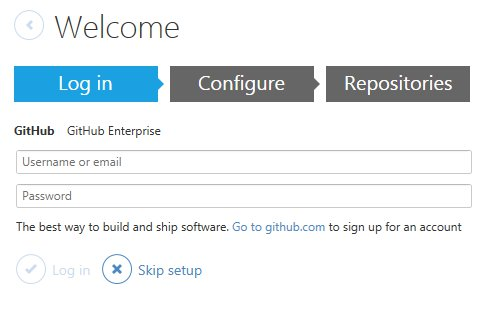
\includegraphics[width=1\textwidth]{2.jpg}
\end{figure}
%
\osoba{Paweł Golonka}
sdsd
dsds

%Paweł Golonka
\osoba{Karol Liszka}%Karol Liszka
\osoba{Bartosz Rusinek}%Bartosz Rusinek


\setcounter{secnumdepth}{-1}


%Gdy mamy dużą bibliografię to możemy wybierać pozycje,
%które cytujemy
%\nocite{ad-tg-80}

%Dodaje wszystkie pozycje z bibliografii
%\nocite{*}

%Po kazdym dodaniu nowej pozycji bibliograficznej
%z katalogu glownego uruchom: bibtex pracadyp
%\bibliographystyle{pdplain}
%\bibliography{tex/pracadyp}

\begin {thebibliography}{11}
\bibitem{Balcerzak2005} Balcerzak J., Pansiuk J.: \emph{Wprowadzenie do kartografii matematycznej}, Warszawa, OWPW~2005.
\bibitem{Barrett} Barrett R. i inni: \emph{Templates for the Solution of Linear Systems: Building Blocks for Iterative Methods1}, wersja elektorniczna Mathematics http://www.siam.org/books.
\bibitem{bjork} Bjork A., Dahlquist G.: \emph{Numerical Methods in Scientific Computing}, Philadelphia, SIAM~2002.
\bibitem{CCITTG4}CCITT, \emph{Facsimile Coding Schemes and Coding Control Functions for Group 4 Facsimile
Apparatus, Recommendation T.6, Volume VII, Fascicle VII.3, Terminal Equipment and
Protocols for Telematic Services, The International Telegraph and Telephone Consultative Committee (CCITT)}, Geneva, CCITT~1985.
\bibitem{drwal:mathematica2000} Drwal G, i in., \emph{Mathematica 4}, Gliwice, WPKJS~200.
\bibitem{Gdowski1982} Gdowski B.: \emph{Elementy geometrii rózniczkowej w zadaniach}, Warszawa, PWN~1982.
\bibitem{Januszewski2006} Januszewski J.: \emph{Systemy satelitarne GPS, Galileo i inne}, Warszawa, PWN~2006.
\bibitem{kielbasinski1992}: Kiełbasiński A., Schwetlick H.: \emph{Numeryczna algebra liniowa}, Warszawa, WNT~1992.
\bibitem{Kincaid2006} Kincaid D.: \emph{Analiza numeryczna}, Warszawa, WNT~2006.
\bibitem{Levine1994} Levine J.: \emph{Programowanie plików graficznych w C/C++}, New York, Wiley~1994.
\bibitem{Longley2006} Longley P. i inni: \emph{GIS teoria i praktyka}, Warszawa, PWN~2006.
\bibitem{GML:opengis} Open Geospatial Consortium Inc.: \emph{OpenGIS Geography Markup Language (GML) Encoding Standard, Version: 3.2.1},  OGC~2007.
\bibitem{GML:opengisimplemntation} Open Geospatial Consortium Inc.: \emph{OpenGIS® Geography Markup Language (GML) Implementation Specification}, OGC~2004.
\bibitem{Opera2002} Opera J.: \emph{Geometria róniczkowa i jej zastosowania}, Warszawa, PWN~2002.
\bibitem{Poczobut1982Geogeza} Odlanicki-Poczobut M.: \emph{Geodezja}, PPWK~1982.
\bibitem{Li2007}Li Y. i inni: \emph{GML Topology Data Storage Schema Design}, Chiba University~2007.
\bibitem{li2004GMLstorage}Li Y., Li J., Zhou S.: \emph{GML Storage}, A Spatial Database Approach,ER (Workshops), str 55-66, 2004.
\bibitem{Sayood2002} Sayood K.: \emph{Kompresja danych}, Warszawa, Rm~2002.
\bibitem{G52003} \emph{The Technical Instruction G-5, The Ground Cadastre and Buildings, The Main Surveying and
Cartographic Bureau}, Warszawa 2003.



\end {thebibliography}


%\listoffigures

%\listoftables 
\end{document}

